\documentclass{report}
\usepackage{graphicx, float}
\usepackage{chapterbib}
\usepackage{fancyhdr}
\usepackage{footmisc}
\renewcommand{\thefootnote}{\fnsymbol{footnote}}
\usepackage{microtype}
\usepackage{appendix}

\pagestyle{fancy}
\fancyhead[R]{UFR STE} % En-tête droite
\fancyfoot[R]{M1 Mathématiques et Applications} % Pied de page droite

\begin{document}
\sloppy


\begin{titlepage}
    \centering
    
\begin{figure}[H]
\begin{minipage}[t]{0.45\linewidth}
\centering

\includegraphics[width =
0.6\linewidth]{logo.jpg}\par\vspace{1cm}

\end{minipage}
\hfill
\begin{minipage}[t]{0.45\linewidth}

\includegraphics[width = 0.4
\linewidth]{lmaa.png}\par\vspace{1cm}

\end{minipage}
\end{figure}
   
    {\scshape\Large Université Des Antilles \par}
    \vspace{1cm}
    {\scshape\Large Master 1 Mathématiques et Applications \par}
     \vspace{1cm}
    {\scshape\Large Année Universitaire 2023-2024 \par}
    \vspace{2cm}
    {\Large\bfseries Rapport de stage : Étude statistique longitudinale de l'influence des facteurs
environnementaux sur la dégradation du chlordécone dans les terres agricoles
martiniquaises (2004-2019). \par}
    \vspace{2cm}
    {\Large\itshape Pierre Chrislin DORIVAL \par}
    \vfill
    Supervisé par\par
    René DORVILLE                 Professeur à l'Université Des Antilles\par
    Pascal ZONGO                  Professeur à l'Université Des Antilles
    \vfill

    % Bottom of the page
    {\scshape\large Du 8 Avril au 8 Juin 2024}
\end{titlepage}

\chapter*{Remerciements}
\addcontentsline{toc}{chapter}{Remerciements}

Je tiens à exprimer ma profonde gratitude à toutes les personnes qui ont contribué à la réalisation de ce stage et de cette étude.

Tout d'abord, je remercie sincèrement mon encadreur, Monsieur René DORVILLE, et mon co-encadreur, Monsieur Pascal ZONGO, pour leur soutien indéfectible, leurs conseils avisés et leur disponibilité tout au long de ce stage. Leur expertise et leur accompagnement m'ont été inestimables pour mener à bien cette recherche.

Je souhaite également adresser mes remerciements aux responsables du master en Martinique, en particulier Monsieur Maximilian HASLER, ainsi qu'au responsable du master, Monsieur Velin JEAN. Un grand merci à Madame Larissa VALMY pour son soutien, notamment pour la convention de stage.

Je remercie également le staff de la scolarité de Martinique et de Guadeloupe pour leur assistance précieuse tout au long de cette période.

Enfin, je tiens à exprimer ma reconnaissance envers ma famille, en particulier ma mère, Jeanne EMMANUEL DORIVAL, et mon père, Joseph Ilioreste DORIVAL, qui ont toujours été à mes côtés. Leur soutien et leur amour ont été des sources constantes de motivation et de réconfort.

Merci à tous.

\tableofcontents
\newpage

\chapter*{Introduction}
\addcontentsline{toc}{chapter}{Introduction}

Selon les ministères français chargés de l’Environnement, de l’Agriculture et de la
Recherche, la Martinique, île des Caraïbes réputée pour sa biodiversité et son agriculture, est confrontée depuis plusieurs décennies à un problème environnemental majeur : la contamination des sols agricoles par le chlordécone ( \cite{sanchez2022chlordecone}). Utilisé massivement dans les plantations de bananes entre les années 1970 et 1993, le chlordécone, pesticide organochloré persistant, persiste dans l'environnement et représente une menace pour la santé publique et la sécurité alimentaire (\cite{coulis2023contamination}).\\

La dégradation du chlordécone dans les sols agricoles est un processus complexe influencé par une multitude de facteurs environnementaux. Comprendre ces facteurs et leur interaction est essentiel pour élaborer des stratégies efficaces de gestion et de décontamination des terres agricoles martiniquaises (\cite{dromard2016assessment}).\\

La présente étude se propose d'explorer en profondeur cette problématique en se concentrant sur les principaux facteurs environnementaux qui influencent la dégradation du chlordécone dans les sols agricoles de la Martinique sur une période de 15 ans. Plus précisément, nous chercherons à répondre à la question suivante : quels sont les facteurs environnementaux qui interagissent pour influencer la dégradation du chlordécone, et comment ces interactions affectent-elles ce processus au fil du temps ?\\

Pour répondre à cette question, nous adopterons une approche multidisciplinaire, combinant des analyses statistiques avancées et une exploration approfondie des données longitudinales sur les niveaux de chlordécone et les variables environnementales pertinentes. Cette approche nous permettra d'identifier les tendances principales, de caractériser les facteurs environnementaux clés et d'évaluer leur impact sur la dégradation du chlordécone dans les sols agricoles martiniquaises.\\

En fin de compte, cette recherche vise à enrichir notre compréhension des processus de dégradation du chlordécone dans un contexte insulaire et tropical, et à fournir des connaissances fondamentales pour orienter les politiques de gestion environnementale et les pratiques agricoles durables dans la région de la Martinique.

\chapter*{État des connaissances sur la dégradation du chlordécone dans les sols agricoles martiniquais.}
\addcontentsline{toc}{chapter}{État des connaissances sur la dégradation du chlordécone dans les sols agricoles martiniquais}

\section*{Effets du chlordécone sur l'environnement et la santé humaine}
\addcontentsline{toc}{section}{Effets du chlordécone sur l'environnement et la santé humaine}
Le chlordécone, un pesticide organochloré largement utilisé dans les plantations de bananes en Martinique jusqu'au début des années 1990, est connu pour ses effets néfastes sur l'environnement et la santé humaine. Des études ont montré sa persistance dans les sols agricoles, son accumulation dans la chaîne alimentaire et son association avec des risques pour la santé, notamment des effets neurotoxiques et cancérigènes chez l'homme.\\


\section*{Processus de dégradation du chlordécone}
\addcontentsline{toc}{section}{Processus de dégradation du chlordécone}


La dégradation du chlordécone dans les sols agricoles est un processus complexe influencé par divers facteurs environnementaux. Les études précédentes (\cite{coulis2023contamination}) ont identifié plusieurs voies de dégradation, notamment la biodégradation par des microorganismes du sol, l'adsorption sur les particules du sol et la dégradation photochimique sous l'effet de la lumière solaire. Cependant, la compréhension de ces processus reste incomplète, en particulier en ce qui concerne leur cinétique et leurs mécanismes exacts.\\


\section*{Facteurs environnementaux influençant la dégradation du chlordécone}
\addcontentsline{toc}{section}{Facteurs environnementaux influençant la dégradation du chlordécone}

Plusieurs études ont examiné l'impact des facteurs environnementaux sur la dégradation du chlordécone dans les sols agricoles. Ces facteurs\footnote{https://sante.gouv.fr/sante-et-environnement/les-plans-nationaux-sante-environnement/article/le-plan-chlordecone-iv-2021-2027} comprennent le type de sol, l'exposition solaire, la température, l'humidité du sol, le pH du sol et la présence de microorganismes dégradateurs. Cependant, les résultats de ces études sont parfois contradictoires, ce qui souligne la nécessité d'une analyse approfondie et intégrée des facteurs environnementaux pour comprendre pleinement leur rôle dans le processus de dégradation du chlordécone.\\


\section*{Lacunes}
\addcontentsline{toc}{section}{Lacunes}

Malgré les progrès réalisés dans la compréhension de la dégradation du chlordécone, plusieurs lacunes subsistent. Ces lacunes incluent le manque de données longitudinales à long terme sur la dégradation du chlordécone dans les sols agricoles de la Martinique, ainsi que l'absence d'études intégrant de manière exhaustive les différents facteurs environnementaux influençant ce processus.
\\
\section*{Conclusion}
\addcontentsline{toc}{section}{Conclusion}
Dans cette section,on met en évidence l'importance cruciale de comprendre les processus de dégradation du chlordécone dans les sols agricoles martiniquaises, ainsi que les facteurs environnementaux qui les influencent. Cette compréhension est essentielle pour élaborer des stratégies efficaces de gestion et de décontamination des terres agricoles contaminées par le chlordécone dans la région de la Martinique.



\chapter*{Méthodologie}
\addcontentsline{toc}{chapter}{Méthodologie}


La méthodologie adoptée dans cette étude est cruciale pour répondre à la problématique posée et atteindre les objectifs fixés. Cette section détaille les données utilisées, les méthodes analytiques appliquées et les étapes suivies pour mener à bien l'analyse des facteurs environnementaux influençant la dégradation du chlordécone dans les sols agricoles de la Martinique sur une période de 15 ans.\\



\section*{Données utilisées}
\addcontentsline{toc}{section}{Données utilisées}

Les données utilisées dans cette étude ont été fournies par le Monsieur Pascal ZONGO, Docteur en mathématiques et professeur à l'Université des Antilles. Elles sont constituées de deux fichiers au format CSV\footnote{Un fichier CSV (en anglais, comma separated values) est le fichier de base des données
recueillies - sans formatage particulier. Chaque champ est séparé par une virgule. } : l'un contenant les données brutes et l'autre contenant les explications sur la signification des données et les définitions des colonnes.\\

Le fichier de données brutes comprend une série temporelle détaillée des niveaux de chlordécone dans les sols agricoles de la Martinique sur une période de 15 ans, de 2004 à 2019. Chaque entrée dans ce fichier représente un échantillon de sol prélevé à un emplacement spécifique, avec des mesures de concentration de chlordécone ainsi que des variables environnementales telles que la pluviométrie, l'exposition solaire, la rugosité du terrain, etc.\\

Le deuxième fichier fournit des explications sur la signification de chaque variable présente dans le fichier de données brutes, ainsi que des définitions des colonnes. Ces informations sont essentielles pour comprendre et interpréter correctement les données, en particulier pour identifier les facteurs environnementaux pertinents qui pourraient influencer la dégradation du chlordécone dans les sols agricoles de la Martinique.\\
 

\section*{Méthodes analytiques}
\addcontentsline{toc}{section}{Méthodes analytiques}


Pour analyser les données longitudinales sur les niveaux de chlordécone et les variables environnementales, plusieurs méthodes analytiques ont été utilisées. Tout d'abord, une analyse statistique descriptive a été réalisée pour explorer les tendances temporelles et spatiales des concentrations de chlordécone dans les sols agricoles de la Martinique. Ensuite, des modèles statistiques adaptés aux données longitudinales ont été appliqués pour évaluer l'impact des facteurs environnementaux sur la dégradation du chlordécone. Ces modèles ont permis de prendre en compte la structure temporelle des données et les interactions entre les différentes variables.
\section*{Logiciel et Packages Utilisés}
\addcontentsline{toc}{section}{Logiciel et Packages Utilisés}

 Dans cette étude, nous avons utilisé le langage de programmation R ( \cite{documentR} ),(\cite{millot2018comprendre}) pour la manipulation des données, l'analyse statistique, et la modélisation. R est un langage puissant et flexible, particulièrement adapté pour les analyses de données complexes et les visualisations. Les packages spécifiques utilisés dans cette étude sont décrits ci-dessous :\\\\
\large\textbf{corrplot :} Créer des graphiques de corrélation pour mieux comprendre les relations entre les variables.\\
\large\textbf{dplyr :} Fournit des outils pour manipuler les données de manière efficace.\\
\large\textbf{nlme :} Ce package permet de réaliser des modèles linéaires mixtes. Ces modèles sont utiles pour analyser les données avec des structures de corrélation et de variabilité complexes, en tenant compte des effets fixes et aléatoires.\\
\large\textbf{lme4 :} Un package similaire à nlme, utilisé pour ajuster des modèles linéaires et non linéaires avec effets mixtes. Il est particulièrement performant pour les grands ensembles de données.\\
\large\textbf{kmeans :} Fonction de base dans R utilisée pour effectuer une analyse de clustering en utilisant l'algorithme K-means. Cet algorithme permet de regrouper les parcelles en fonction de leurs caractéristiques similaires.\\
\large\textbf{dtwclust :} Ce package permet la réalisation de clustering sur des séries temporelles en utilisant des distances dynamiques de type DTW (Dynamic Time Warping), utile pour analyser les profils de dégradation au fil du temps.\\
\large\textbf{ggplot2 :} Un package de visualisation de données basé sur la grammaire des graphiques. Il permet de créer des visualisations élégantes et complexes de manière simple et intuitive.\\
\large\textbf{reshape2 :} Utilisé pour réorganiser les données (par exemple, pour passer d'un format large à un format long), facilitant ainsi l'analyse et la visualisation.
\\\\
En plus de R, nous avons également utilisé Microsoft Power BI ( \cite{power} ), un outil puissant de business intelligence et de visualisation de données. Power BI nous a permis de créer des tableaux de bord interactifs et des graphiques dynamiques pour explorer et présenter les résultats de manière claire et intuitive.
\\

\section*{Stratégies d'évaluation des résultats}
\addcontentsline{toc}{section}{Stratégies d'évaluation des résultats}

Dans cette section, nous examinerons les stratégies utilisées pour évaluer les résultats de notre étude sur la dégradation du chlordécone dans les sols agricoles de la Martinique. Les stratégies d'évaluation comprennent généralement une combinaison de mesures quantitatives et qualitatives pour évaluer la pertinence et la fiabilité des résultats obtenus. Voici quelques stratégies clés que nous pourrions utiliser :\\\\
\large\textbf{Analyse des tendances temporelles} \\
Nous analyserons les tendances temporelles des niveaux de chlordécone dans les sols agricoles au fil des années pour identifier toute évolution significative dans la dégradation du chlordécone. Cela pourrait inclure l'utilisation de graphiques de séries chronologiques pour visualiser les changements au fil du temps.\\

\large\textbf{Analyse des corrélations}\\
Nous examinerons les corrélations entre les niveaux de chlordécone et les variables environnementales telles que la pluviométrie, l'ensoleillement, la rugosité du terrain, etc. Cela nous aidera à déterminer les facteurs qui influencent le processus de dégradation du chlordécone.\\\\
\large\textbf{Validation des clusters et des classifications}\\
 Nous utiliserons des techniques de clustering ou de classification pour regrouper les parcelles en fonction de leurs profils de dégradation, nous évaluerons la validité de ces groupes en utilisant des mesures telles que l'indice de Davies-Bouldin ou l'indice de silhouette\footnote{En partitionnement de données (clustering), le coefficient de silhouette est une mesure de qualité d'une partition d'un ensemble de données en classification automatique}. Cela nous aidera à déterminer la cohérence et la qualité des regroupements obtenus.\\\\
\large\textbf{Analyse de sensibilité}\\
 Nous effectuerons une analyse de sensibilité pour évaluer la robustesse de nos résultats par rapport à différentes hypothèses ou paramètres utilisés dans notre analyse. Cela nous permettra de déterminer la stabilité de nos conclusions face à des variations potentielles dans les méthodes ou les données utilisées.\\\\
\large\textbf{Consultation des documents}\\
Enfin, nous pourrions consulter des documents du ministère de la Santé publique ,les études et les publications publiés par le ministère de la Santé publique de la Martinique. Ces documents peuvent contenir des informations précieuses sur la contamination par le chlordécone, ses effets sur la santé publique et les efforts de gestion de cette pollution..\\
 
En utilisant une combinaison de ces stratégies, nous serons en mesure d'évaluer de manière approfondie les résultats de notre étude sur la dégradation du chlordécone dans les sols agricoles de la Martinique. Cela nous permettra d'obtenir des conclusions robustes et fiables qui pourront éclairer les pratiques de gestion environnementale dans la région.

\section*{Analyse statistiques descriptive}
\addcontentsline{toc}{section}{Analyse statistiques descriptive}

En combinant les techniques d'analyse descriptive, nous allons obtenir un aperçu complet des données sur la dégradation du chlordécone dans les sols agricoles de la Martinique, ce qui nous permettra de mieux comprendre les caractéristiques et les tendances des données avant de passer à des analyses plus avancées.\\

La description du taux de chlordécone révèle une gamme de valeurs étendue, allant de 0.0010 à 17.350. Le premier quartile (Q1) de cette distribution est de 0.0011, indiquant que 25\% des observations ont un taux de chlordécone inférieur ou égal à cette valeur. La médiane, qui représente la valeur centrale de la distribution, est de 0.0033. La moyenne du taux de chlordécone est de 0.5607, ce qui suggère une tendance vers des valeurs plus élevées en raison de la présence possible de valeurs aberrantes. Le troisième quartile (Q3) est de 0.2167, indiquant que 75\% des observations ont un taux de chlordécone inférieur ou égal à cette valeur. Ces statistiques mettent en évidence une forte variabilité dans les niveaux de chlordécone dans les sols agricoles de la Martinique, avec une tendance vers des valeurs plus élevées dans les quartiles supérieurs.\\


\section*{Nombre de prélèvements de taux de chlordécone par commune.}
\addcontentsline{toc}{section}{Nombre de prélèvements de taux de chlordécone par commune.}


Selon les résultats, environ 21 000 prélèvements ont été effectués sur 35 communes. La répartition de ces prélèvements est inégale, avec une concentration notable dans les communes de MORNE-ROUGE, SAINT-JOSEPH, GROS-MORNE, et LAMENTIN, entre autres. Cette distribution déséquilibrée indique une surreprésentation de certaines zones par rapport à d'autres dans l'étude des niveaux de chlordécone. De plus, il y avait de nombreuses difficultés à mener des études longitudinales sur les parcelles, car il n'y a pas beaucoup de parcelles où des prélèvements ont été faits sur des années différentes. En effet, pour la majorité des parcelles, les prélèvements ont été effectués plusieurs fois sur une seule année, ce qui limite l'analyse temporelle de la dégradation du chlordécone.

\begin{figure}[H]
\centering
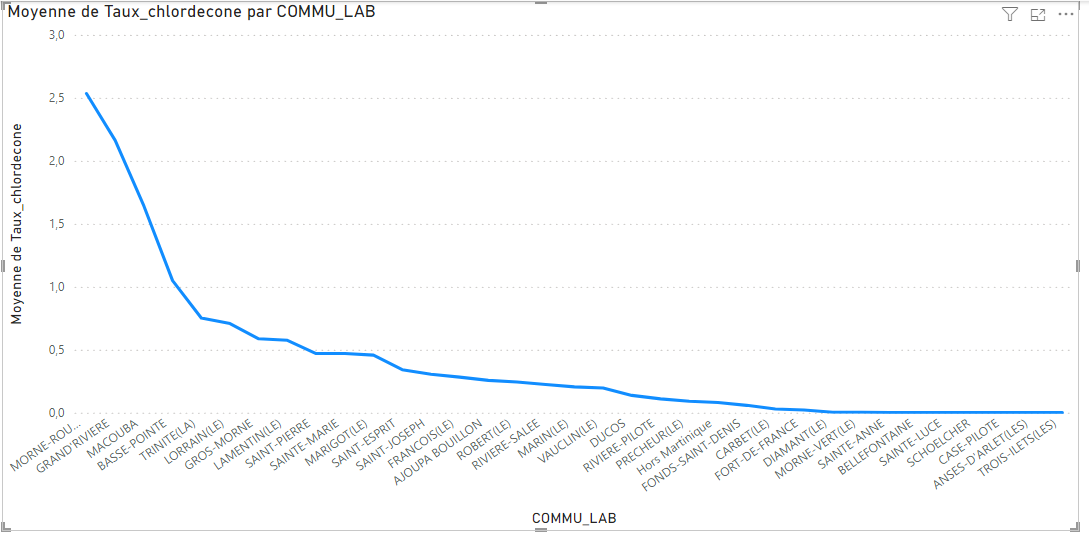
\includegraphics[width = 1
\linewidth]{moyenne_taux_chlordecone_par_commune.png}
\caption{Moyenne de Taux de Chlordécone par commune}
\end{figure}

\begin{figure}[H]
\centering
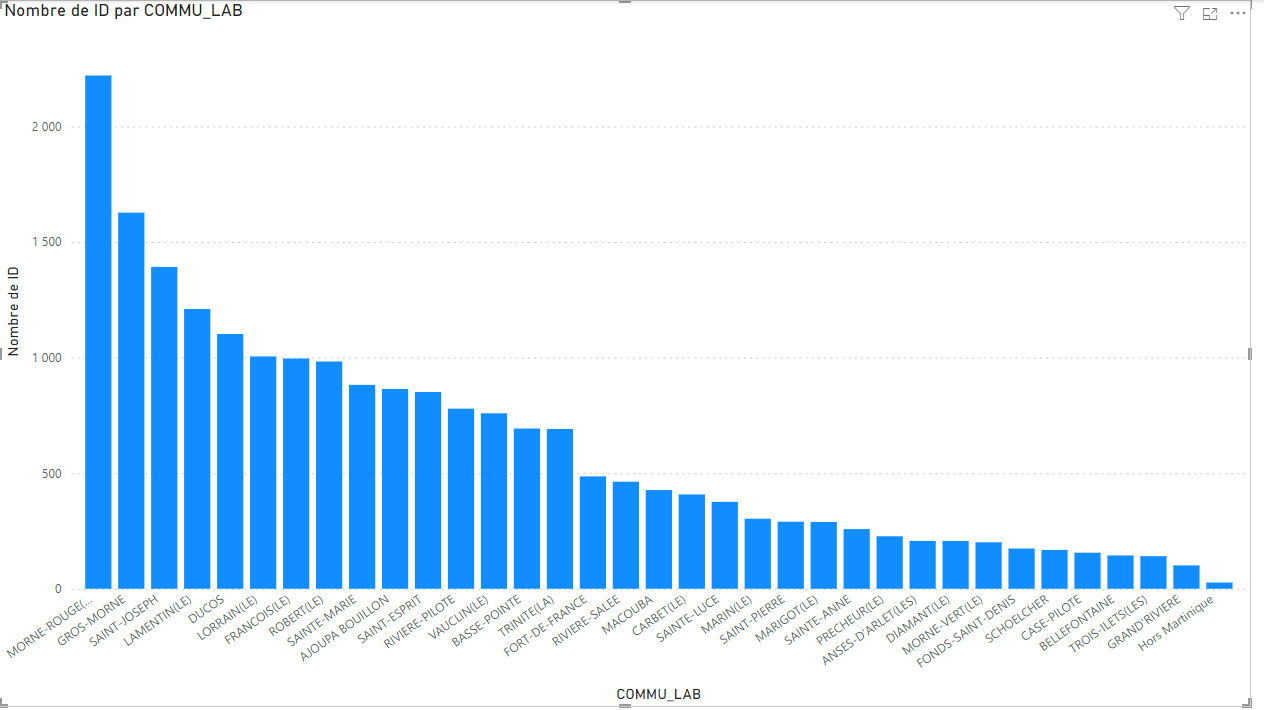
\includegraphics[width = 1
\linewidth]{nombre_prel_par_commune.png}
\caption{Nombre de prélèvement par commune}
\end{figure}
 
\section*{Identification des tendances principales dans la dégradation du chlordécone }
\addcontentsline{toc}{section}{Identification des tendances principales dans la dégradation du chlordécone}

Vérification de la normalité des résidus et  création d'un modèle de régression linéaire multiple (\cite{statistic1})avec les variables environnementales:\\  
Description du Modèle de Régression Linéaire Multiple\\
\large\textbf{Objectif :} Créer un modèle de régression linéaire multiple pour prédire le Taux de Chlordécone à partir de variables environnementales.\\
\Large\textbf{Variable dépendante :}\\
\large\textbf{Taux\_chlordecone :} La variable dépendante qu'on essaie de prédire.\\
\large\textbf{Variables indépendantes :}\\
\large\textbf{moyenne\_pulviometrie :} Moyenne des précipitations sur les sols.\\
\large\textbf{mnt.exposition\_mean :} Direction horizontale de la pente du terrain en degrés.\\
\large\textbf{mnt.ombrage\_mean :} Aspect des ombres du terrain.\\
\large\textbf{mnt.pente\_mean :} Inclinaison de la pente en degrés.\\
\large\textbf{mnt.tpi\_mean :} Indice de position topographique.\\

Sur le logiciel R on utilise les commandes qqnorm(resid(modele)) et qqline(resid(modele)) qui sont utilisées pour visualiser les résidus du modèle de régression. Elles créent un graphique Q-Q (quantile-quantile) \cite{millot2018comprendre} qui permet d'évaluer si les résidus suivent une distribution normale. Voici le graphique:

\begin{figure}[H]
\centering
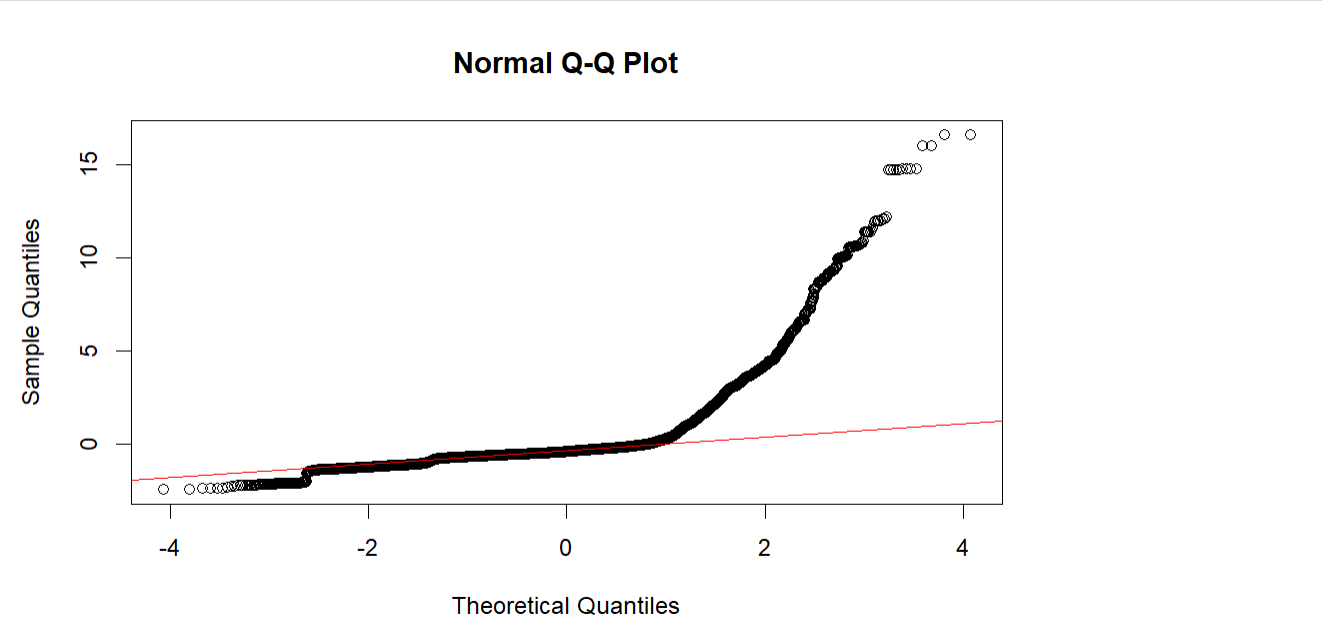
\includegraphics[width = 1
\linewidth]{graphiqueQQ.png}
\caption{Graphique Q-Q}
\end{figure}

Le graphique Q-Q (quantile-quantile) indique que les résidus ne sont pas normalement distribués. Les points qui dévient de manière significative de la ligne suggèrent que les résidus ne suivent pas une distribution normale. 
Cela peut signaler plusieurs problèmes potentiels, notamment :\\
Variabilité non constante (hétéroscédasticité) : Les variances des résidus peuvent ne pas être homogènes à travers les observations, ce qui viole une des hypothèses de base de la régression linéaire.
Les valeurs aberrantes peuvent déformer la distribution des résidus.\\

Ces déviations par rapport à la normalité des résidus peuvent affecter la validité des inférences statistiques dérivées du modèle. Il est donc important d'identifier et de traiter ces problèmes pour améliorer la qualité et la fiabilité du modèle.\\

Pour vérifier Ces déviations par rapport à la normalité des résidus, on a tracé un histogramme des résidus.  \\
Voir le schéma  ci-dessous :\\


\begin{figure}[H]
\centering
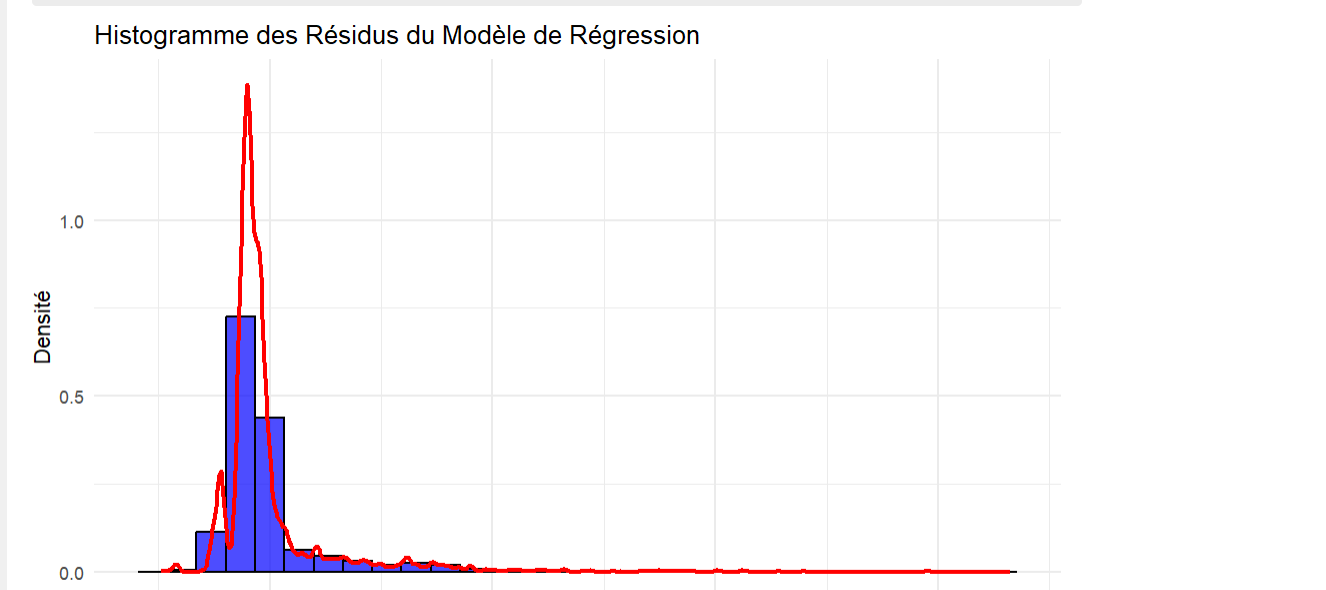
\includegraphics[width = 1
\linewidth]{regression.png}
\caption{Histogramme des Résidus du Modèle de Régression}
\end{figure}

\begin{figure}[H]
\centering
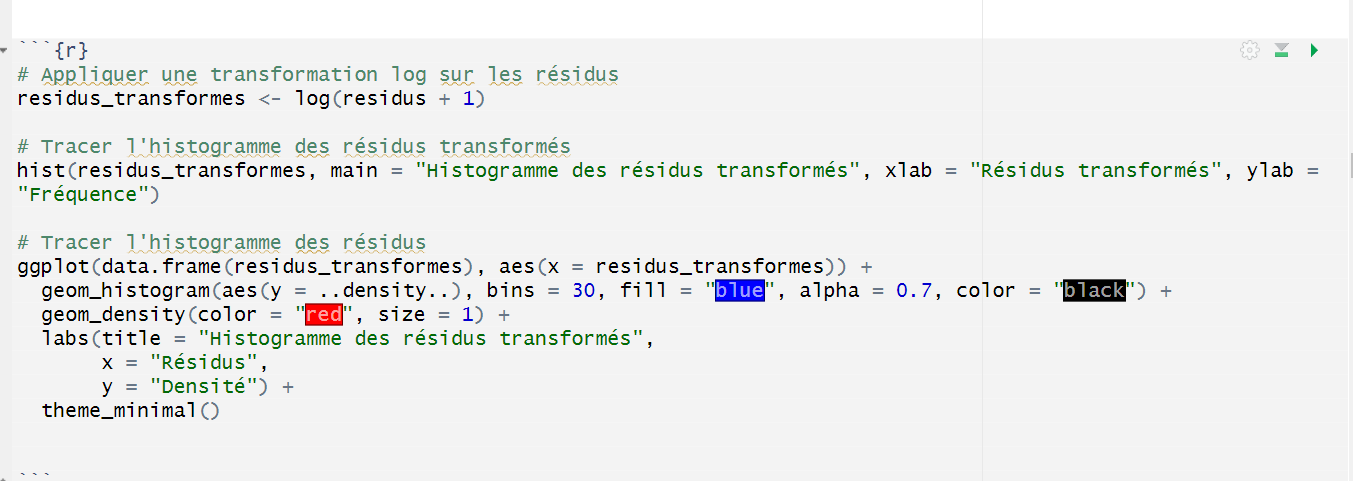
\includegraphics[width = 1
\linewidth]{logresidus.png}
\caption{Code de Transformation log}
\end{figure}


On a constaté que la distribution des résidus est asymétrique dans l'histogramme, pour résoudre ce problème on a appliqué une transformation logarithmique aux données pour rendre la distribution des résidus plus proche de la normalité.\\
\begin{figure}[H]
\centering
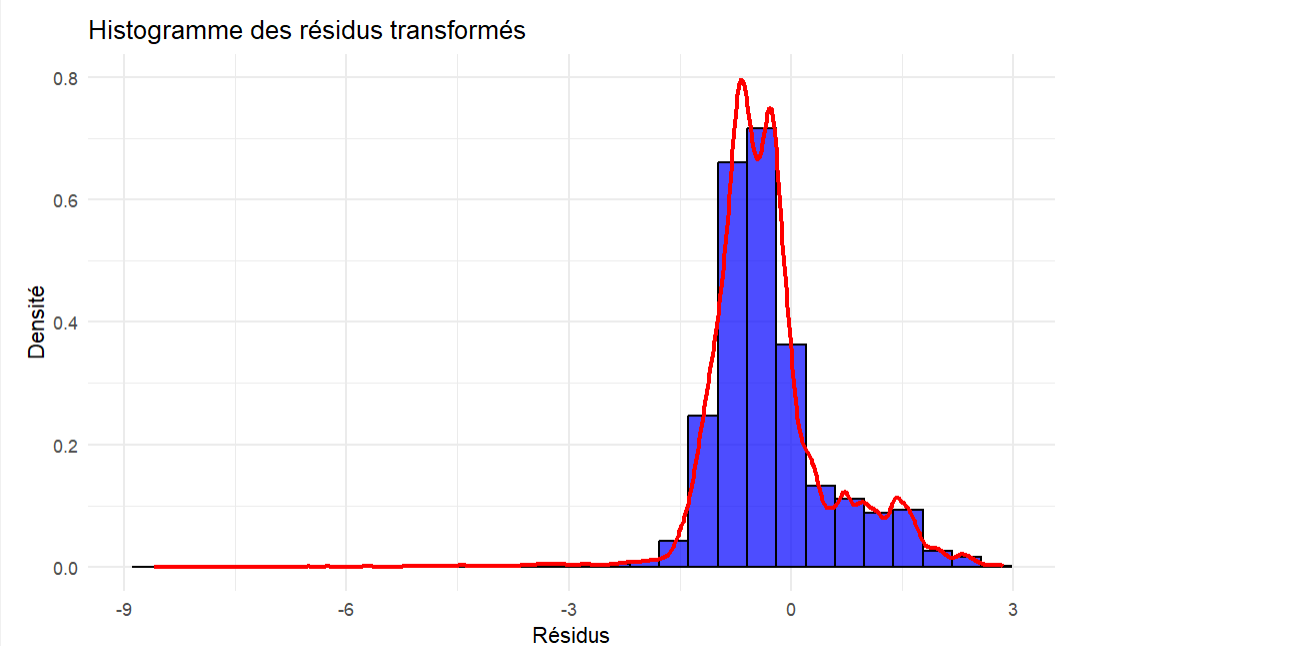
\includegraphics[width = 1
\linewidth]{residustransf.png}
\caption{Histogramme des résidus transformés}
\end{figure}

On constate que la distribution est toujours asymétrique, pour faire suite avec notre analyse on a appliqué le test de Levene\footnote{https://ontostats.univ-paris8.fr/omk/s/logicielsStats/item/6954} \cite{o2002levene} pour vérifier l'homoscédasticité des résidus transformés:\\
 

\begin{figure}[H]
\centering
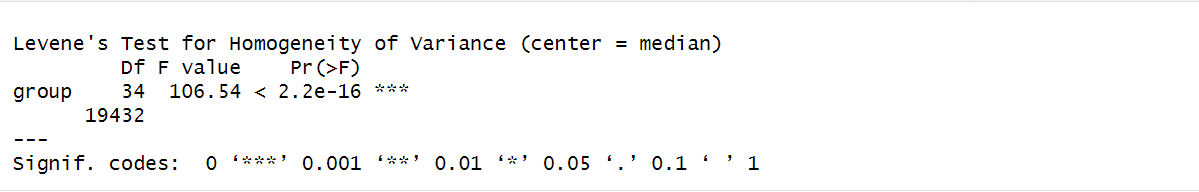
\includegraphics[width = 1
\linewidth]{leneve.png}
\caption{resultat test Leneve}\label{leneve}
\end{figure}

\Large\textbf{Interprétation des Résultats du Test de Levene et Analyse des Corrélations}\\
Le résultat du test de Levene ( figure \ref{leneve}) pour l'homogénéité des variances indique une forte significativité statistique avec une valeur p très faible, inférieure à 2.2e-16 (ce qui signifie essentiellement que la valeur p est très proche de zéro).\\

Cela suggère qu'il y a des différences significatives entre les variances des résidus entre les groupes (niveaux de la variable indépendante). En d'autres termes, l'hypothèse nulle d'homoscédasticité est rejetée, ce qui signifie que les variances des résidus ne sont pas constantes à travers tous les niveaux de la variable indépendante.\\

Les résultats du test de Levene indiquent une hétéroscédasticité significative, ce qui peut remettre en question l'interprétation des résultats de l'ANOVA. Lorsque l'hypothèse d'homoscédasticité est violée, les conclusions tirées des tests statistiques classiques peuvent ne pas être fiables. Dans ce contexte, il est souvent recommandé d'utiliser des méthodes alternatives qui ne reposent pas sur cette hypothèse, comme les tests robustes, ou d'envisager des transformations supplémentaires des données pour stabiliser les variances.\\

Cependant, en raison de contraintes de temps et de ressources, nous ne pouvons pas poursuivre des recherches analytiques avancées pour le moment. Nous allons donc nous concentrer sur une analyse des corrélations entre chaque variable indépendante et le taux de chlordecone de manière séparée. Cela nous permettra de comprendre comment chaque variable individuelle est liée au taux de chlordécone sans nécessiter des techniques statistiques avancées.\\


\section*{Visualisation des Corrélations}
\addcontentsline{toc}{section}{Visualisation des Corrélations}

Nous créerons des graphiques de dispersion pour visualiser les relations entre le taux de chlordécone et chaque variable indépendante.\\

\Large\textbf{Interprétation des Résultats}\\
En analysant les coéfficients de corrélation et les graphiques de dispersion, nous pourrons identifier les variables environnementales qui ont la plus forte association linéaire avec le taux de chlordecone. Les variables présentant des corrélations significatives et des relations visuelles claires seront considérées comme les plus influentes.\\


\begin{figure}[H]
\centering
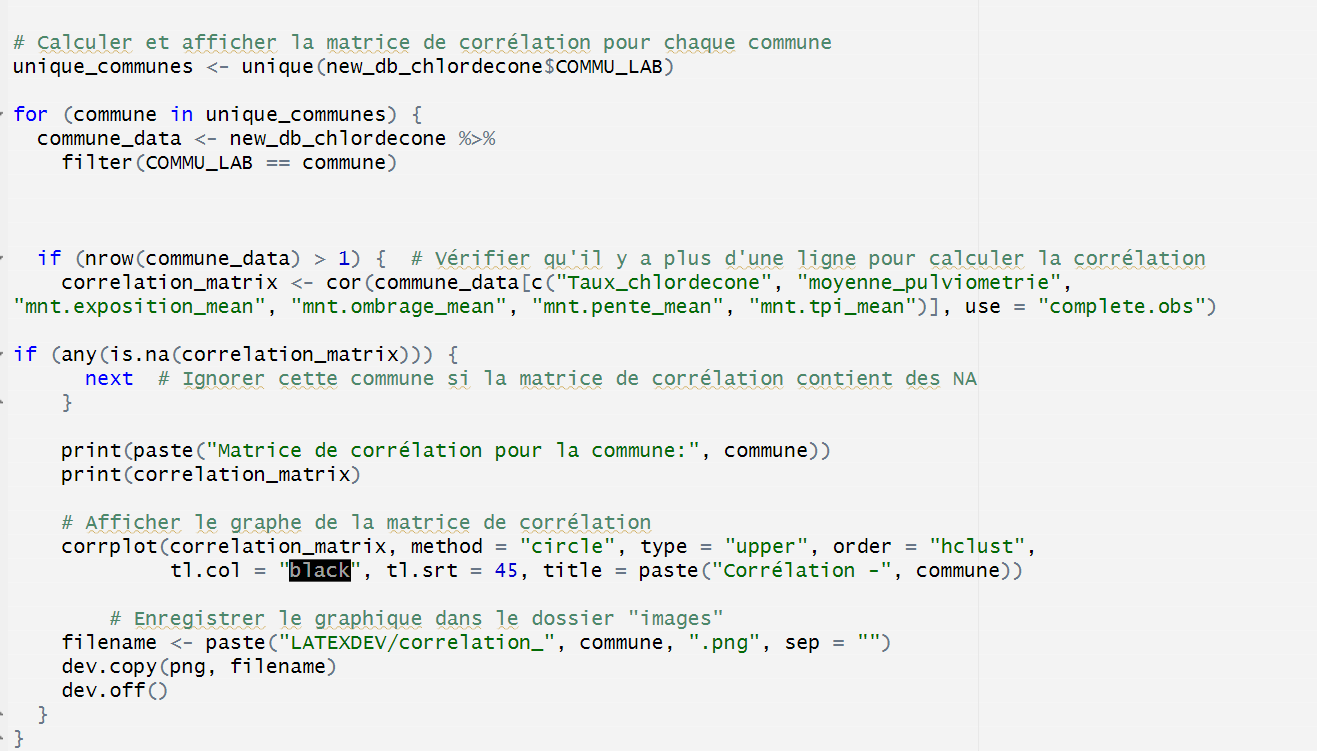
\includegraphics[width = 1
\linewidth]{codecorr.png}
\caption{Code calcul corrélation}
\end{figure}

\begin{figure}[H]
\begin{minipage}[t]{0.45\linewidth}
\centering
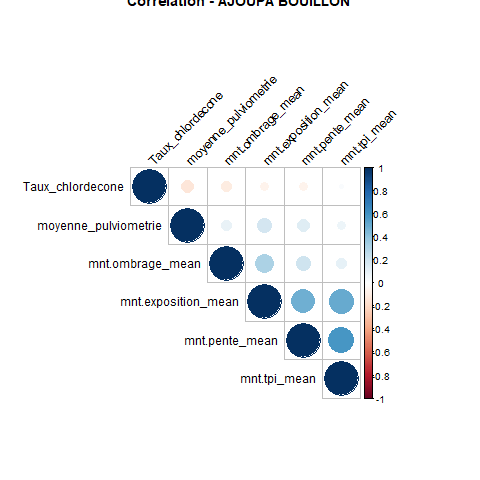
\includegraphics[width =
0.6\linewidth]{correlation_AJOUPA_BOUILLON.png}
\caption{correlation AJOUPA BOUILLON}
\end{minipage}
\hfill
\begin{minipage}[t]{0.45\linewidth}
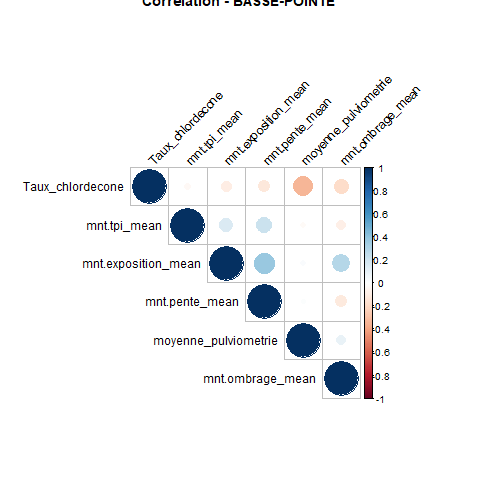
\includegraphics[width = 0.6
\linewidth]{correlation_BASSE-POINTE.png}
\caption{correlation BASSE-POINTE}
\end{minipage}
\end{figure}

\begin{figure}[H]
\begin{minipage}[t]{0.45\linewidth}
\centering
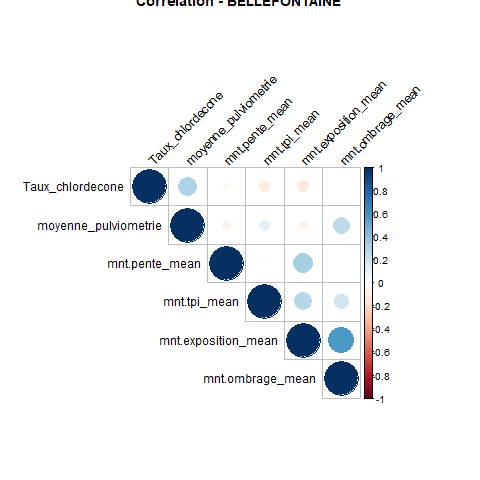
\includegraphics[width =
0.6\linewidth]{correlation_BELLEFONTAINE.png}
\caption{correlation BELLEFONTAINE}
\end{minipage}
\hfill
\begin{minipage}[t]{0.45\linewidth}
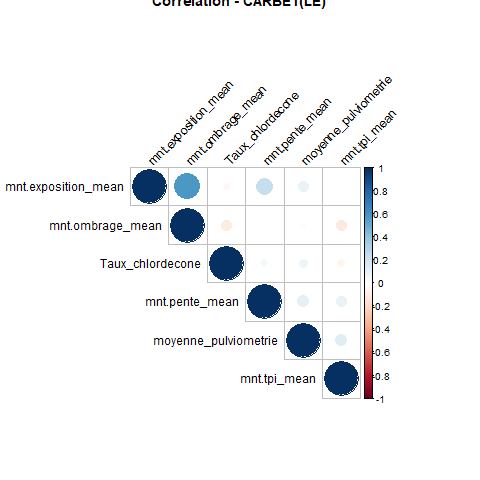
\includegraphics[width = 0.6
\linewidth]{correlation_CARBET(LE).png}
\caption{correlation CARBET}
\end{minipage}
\end{figure}

\begin{figure}[H]
\begin{minipage}[t]{0.45\linewidth}
\centering
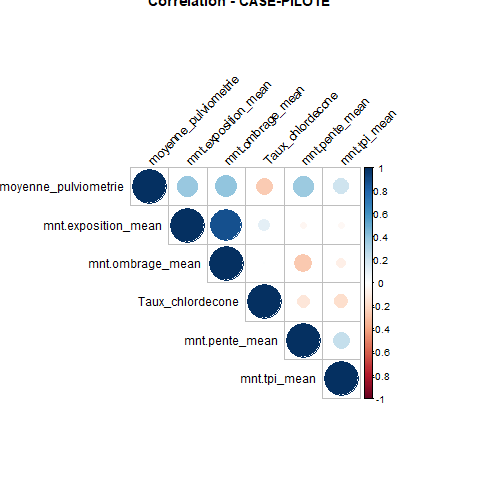
\includegraphics[width =
0.6\linewidth]{correlation_CASE-PILOTE.png}
\caption{correlation CASE-PILOTE}
\end{minipage}
\hfill
\begin{minipage}[t]{0.45\linewidth}
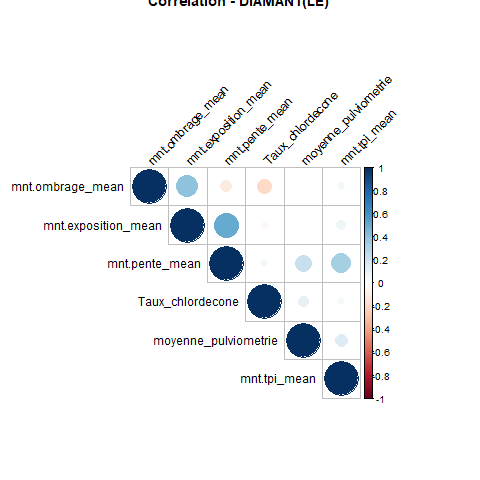
\includegraphics[width = 0.6
\linewidth]{correlation_DIAMANT(LE).png}
\caption{correlation DIAMANT}
\end{minipage}
\end{figure}


\begin{figure}[H]
\begin{minipage}[t]{0.45\linewidth}
\centering
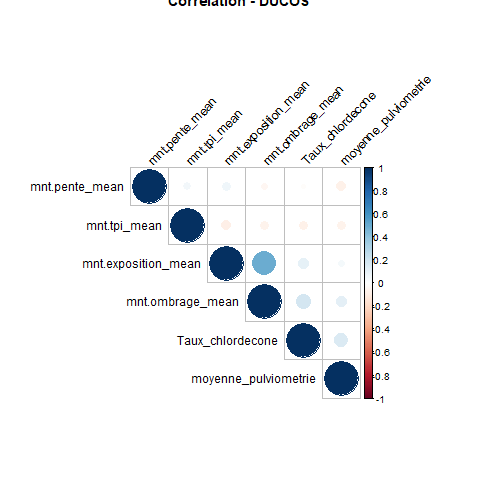
\includegraphics[width =
0.6\linewidth]{correlation_DUCOS.png}
\caption{correlation DUCOS}
\end{minipage}
\hfill
\begin{minipage}[t]{0.45\linewidth}
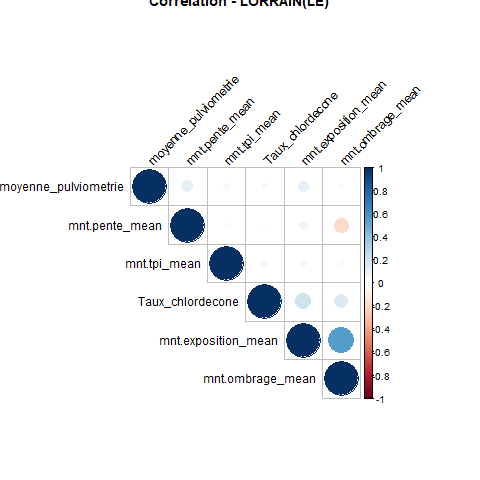
\includegraphics[width = 0.6
\linewidth]{correlation_LORRAIN(LE).png}
\caption{correlation LORRAIN}
\end{minipage}
\end{figure}

\begin{figure}[H]
\begin{minipage}[t]{0.45\linewidth}
\centering
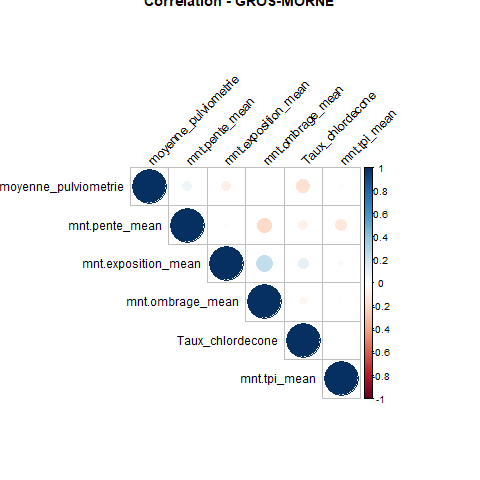
\includegraphics[width =
0.6\linewidth]{correlation_GROS-MORNE.png}
\caption{correlation GROS-MORNE}
\end{minipage}
\hfill
\begin{minipage}[t]{0.45\linewidth}
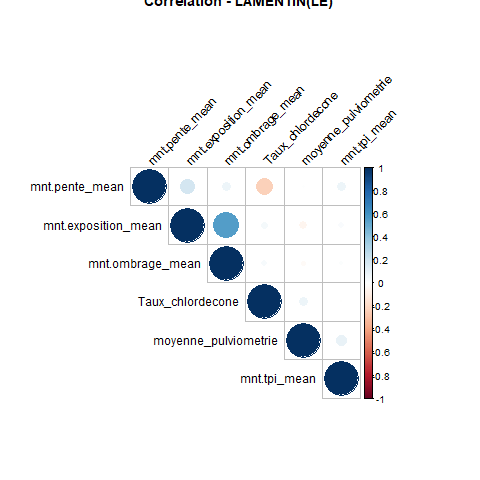
\includegraphics[width = 0.6
\linewidth]{correlation_LAMENTIN(LE).png}
\caption{correlation LAMENTIN}
\end{minipage}
\end{figure}


\begin{figure}[H]
\begin{minipage}[t]{0.45\linewidth}
\centering
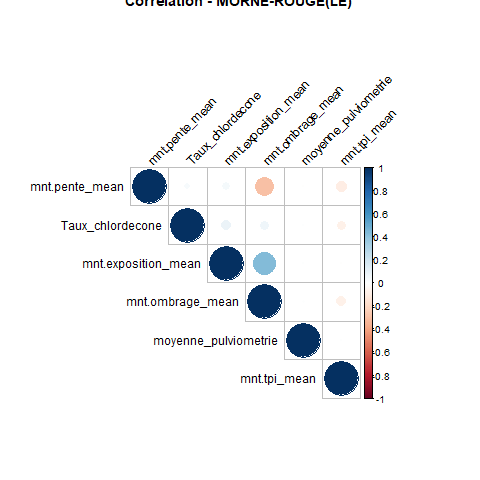
\includegraphics[width =
0.6\linewidth]{correlation_MORNE-ROUGE(LE).png}
\caption{correlation MORNE-ROUGE}
\end{minipage}
\hfill
\begin{minipage}[t]{0.45\linewidth}
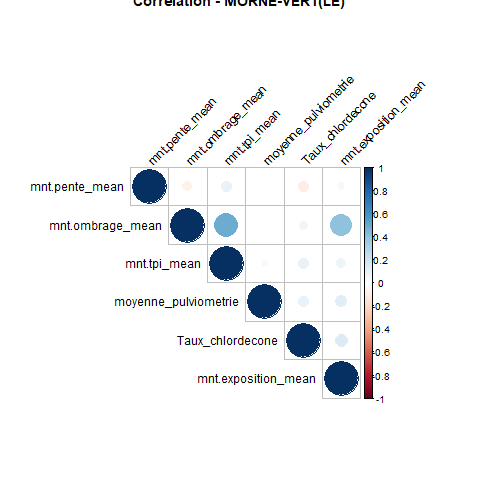
\includegraphics[width = 0.6
\linewidth]{correlation_MORNE-VERT(LE).png}
\caption{correlation MORNE-VERT}
\end{minipage}
\end{figure}

Ainsi, nous avons constaté une forte concentration de chlordécone dans les communes du nord de l'Atlantique, telles que Morne-Rouge, Gros-Morne, et Le Lorrain. Le taux de chlordécone a également diminué au fil des années. Cette réduction est également observée dans différentes communes de l'île. \\

On observe dans des communes comme Basse-Pointe, une forte réduction du taux de chlordécone. Cette réduction est due à plusieurs facteurs, notamment sa situation géographique avec une pente importante. La pluviométrie élevée dans cette zone entraîne un fort ruissellement, qui transporte le chlordécone. De plus, étant soluble dans l'eau, le chlordécone subit un phénomène de dissolution. L'exposition du sol joue également un rôle dans la réduction du taux de chlordécone grâce à des phénomènes de dégradation naturelle.\\
\section*{Analyse Clustering}
\addcontentsline{toc}{section}{Analyse Clustering}

Pour séparer les parcelles en catégories selon leur taux de contamination de chlordécone à l'aide d'un clustering, on a utilisé l'algorithme K-means. Voici les resultats: \\

\begin{figure}[H]
\centering
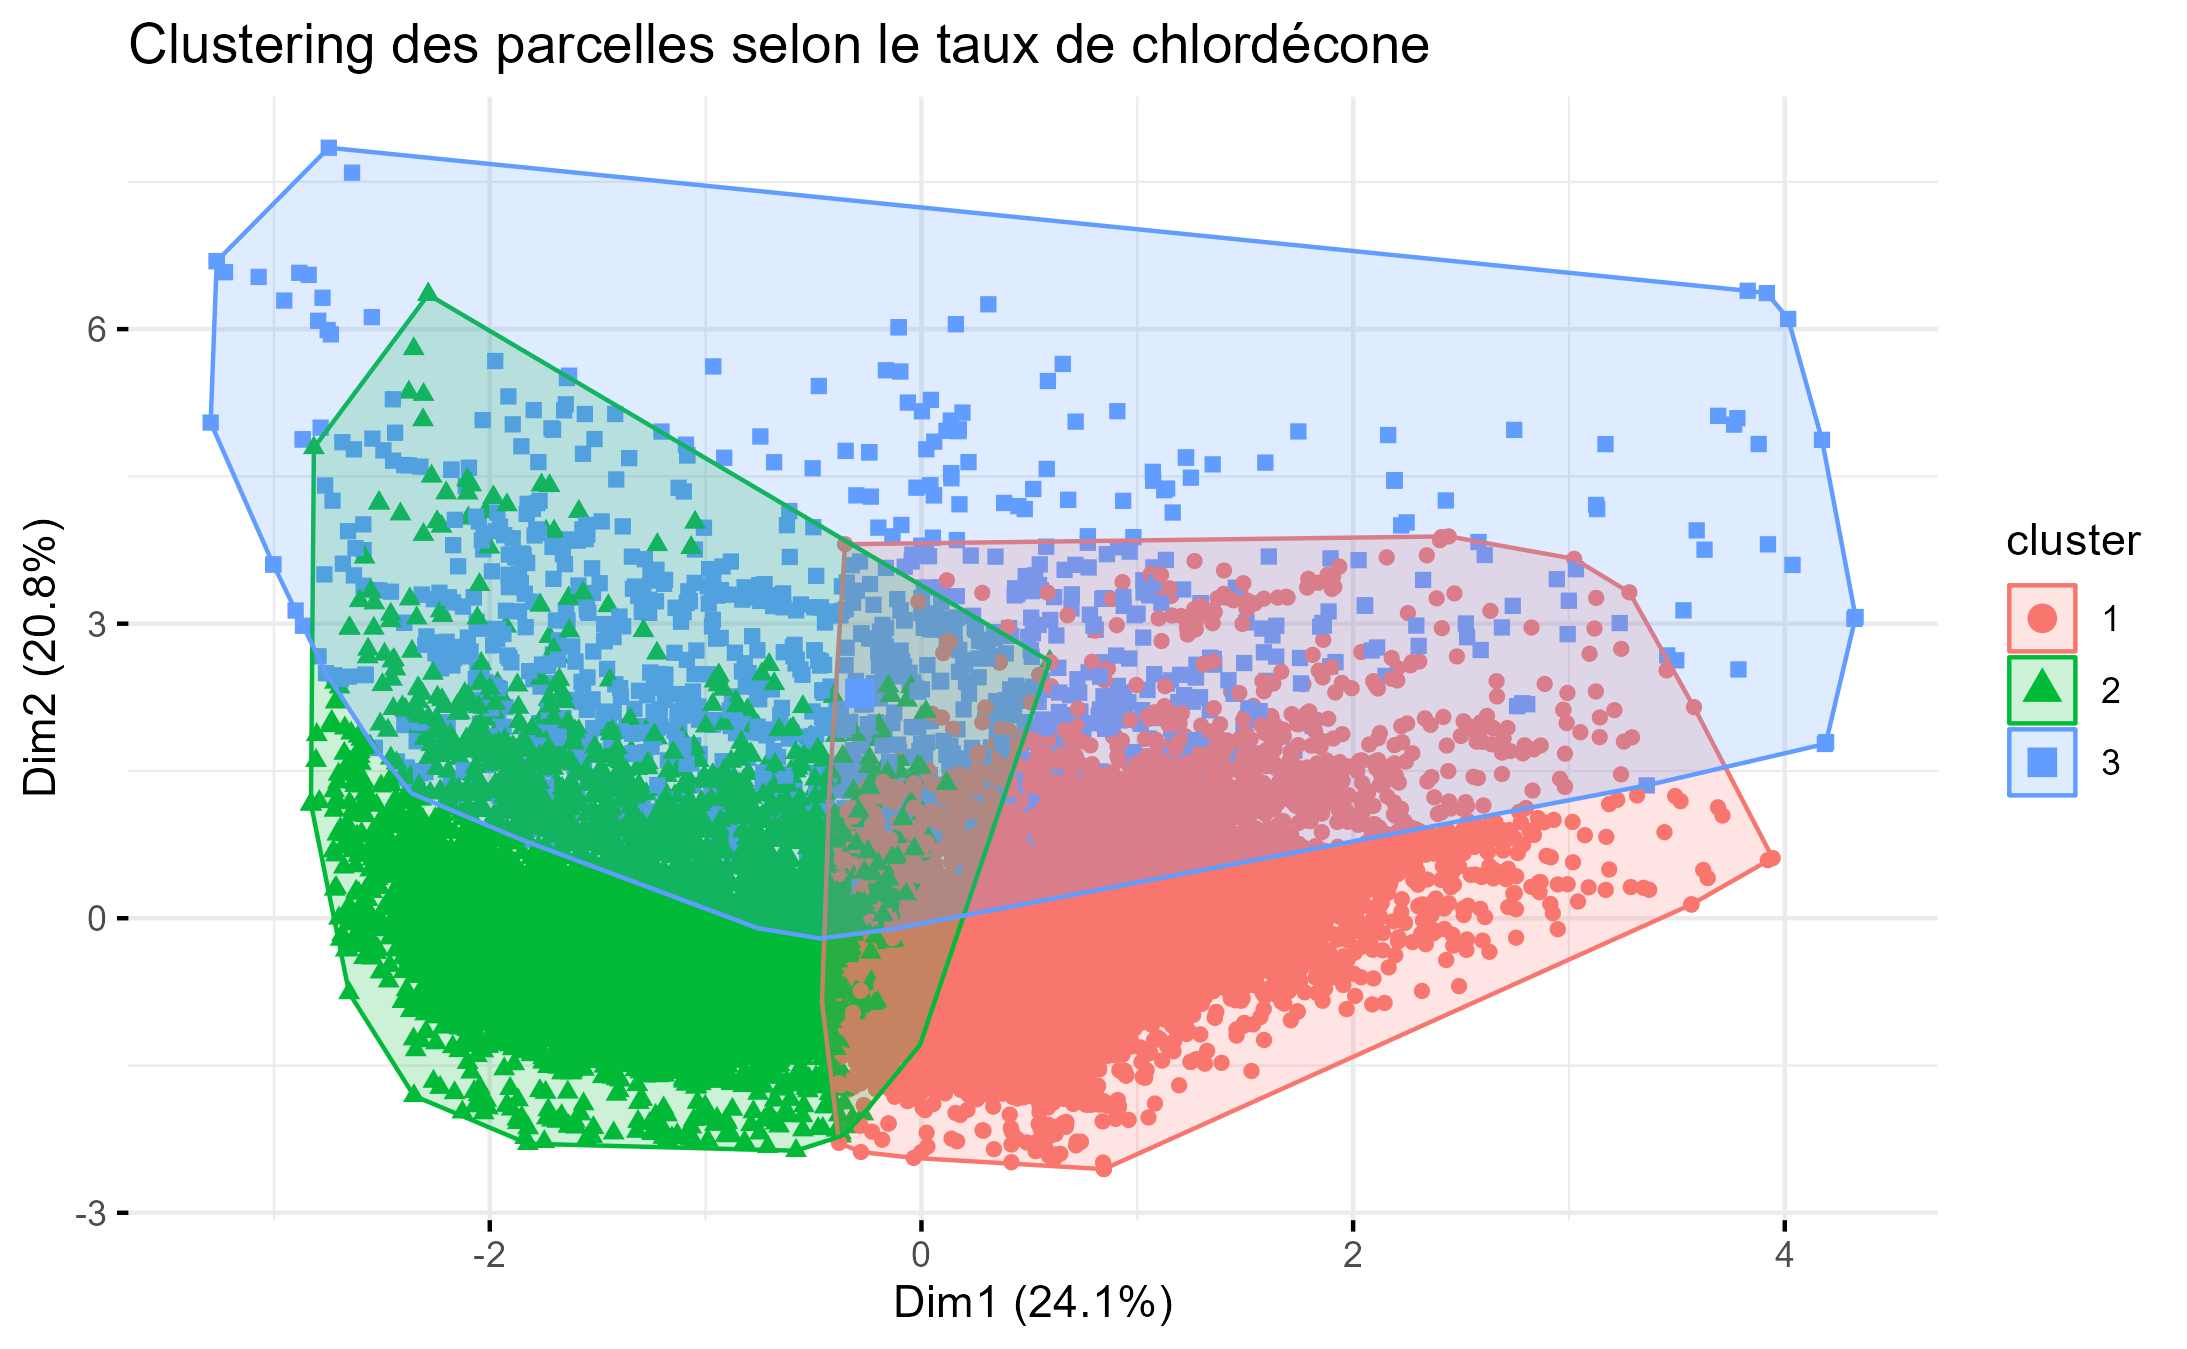
\includegraphics[width = 1
\linewidth]{clusters_parcelles.png}
\caption{Clustering des parcelles selon le taux de chlordécone}
\end{figure}

\begin{figure}[H]
\centering
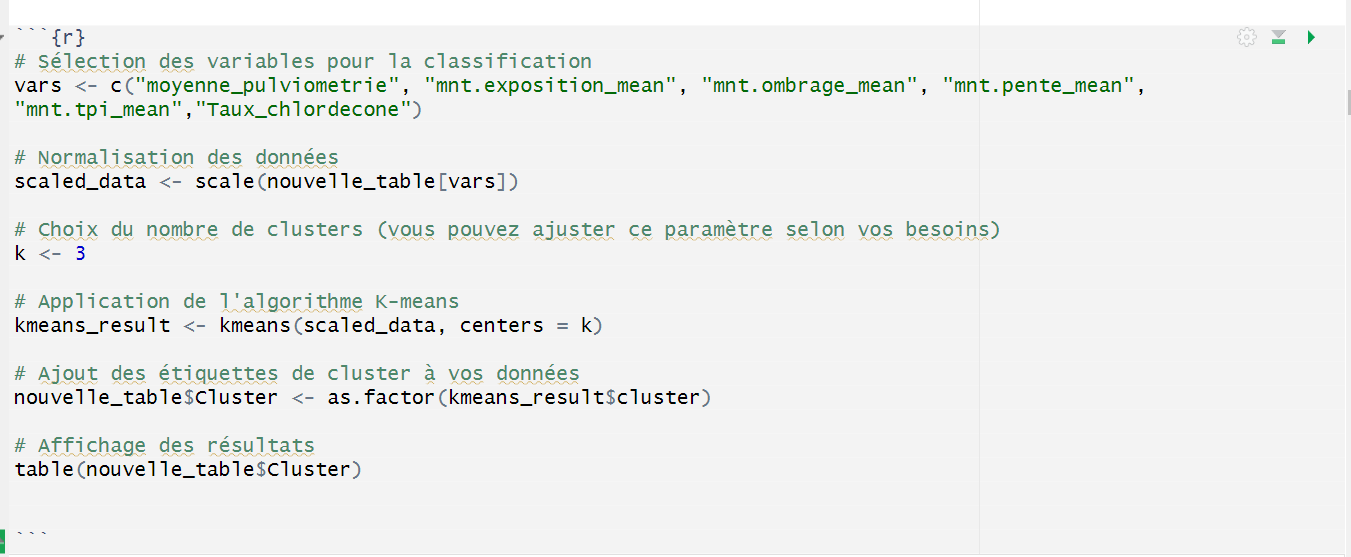
\includegraphics[width = 1
\linewidth]{codecluster1.png}
\caption{Code R K-means}
\end{figure}

\Large\textbf{Une descrption de chaque cluster en termes des variables.}\\
\large\textbf{Cluster 1 :} Les parcelles dans ce cluster ont un taux de chlordécone moyen élevé, une moyenne pluviométrique faible, etc.\\
\large\textbf{Cluster 2 :} Les parcelles dans ce cluster ont un taux de chlordécone moyen faible, une moyenne pluviométrique élevée, etc.\\
\large\textbf{Cluster 3 :} Les parcelles dans ce cluster ont des valeurs intermédiaires pour toutes les variables.\\

Les clusters nous permettent de regrouper les parcelles en fonction de leur taux de contamination par la chlordécone et de leurs caractéristiques environnementales. Cela aide à cibler les interventions et les analyses futures sur les parcelles les plus contaminées.\\
 

\section*{Analyse des résultats}
\addcontentsline{toc}{section}{Analyse des résultats}

L'analyse des résultats obtenus à partir des prélèvements de taux de chlordécone révèle plusieurs tendances et informations importantes pour la gestion de la contamination des sols agricoles. Environ 21 000 prélèvements ont été effectués sur 35 communes, mais la répartition de ces prélèvements est inégale, avec une concentration notable dans les communes de MORNE-ROUGE, SAINT-JOSEPH, GROS-MORNE, et LAMENTIN. Cette distribution déséquilibrée suggère une surreprésentation de certaines zones, ce qui peut biaiser les conclusions tirées à l'échelle régionale.\\

\section*{Défis et limitations}
\addcontentsline{toc}{section}{Défis et limitations}

Un défi majeur rencontré lors de l’étude est l'inégale répartition des prélèvements au fil des années sur les différentes parcelles. La majorité des prélèvements ont été effectués plusieurs fois sur une seule année, ce qui complique l'analyse longitudinale des tendances de dégradation du chlordécone. Cette limitation pourrait potentiellement réduire la précision des modèles de dégradation temporelle, car il manque des données continues et récurrentes sur une période prolongée pour de nombreuses parcelles.\\

De plus, la concentration des prélèvements dans certaines communes limite la généralisation des résultats. Une étude plus équilibrée et extensive nécessiterait une couverture géographique plus uniforme pour éviter les biais de surreprésentation.\\

\large\textbf{Implications pour la gestion des sols contaminés.}\\

Les résultats de cette étude ont des implications directes pour la gestion des sols contaminés par le chlordécone. En identifiant les zones avec des rythmes de décontamination différents et les facteurs environnementaux associés, il est possible de développer des stratégies de gestion plus ciblées. Par exemple, les parcelles avec des conditions favorisant une dégradation plus lente pourraient nécessiter des interventions plus intensives ou des méthodes de remédiation spécifiques.
\\\\
\large\textbf{Les recommandations pour la gestion et la décontamination des terres agricoles pourraient inclure :}\\
\large\textbf{Augmentation de la fréquence des prélèvements :} Assurer une couverture temporelle plus homogène des prélèvements pour permettre une meilleure analyse longitudinale.\\
\large\textbf{Extension de la couverture géographique :} Équilibrer les prélèvements entre toutes les communes pour éviter les biais de surreprésentation.\\
\large\textbf{Interventions ciblées :} Développer des stratégies spécifiques pour les zones identifiées comme ayant des taux de dégradation plus lents.\\\\
\Large\textbf{Perspectives pour les recherches futures}\\

Les résultats de cette étude ouvrent plusieurs avenues pour les recherches futures. Une approche multidisciplinaire intégrant des experts en agronomie, climatologie, et géostatistique pourrait affiner les modèles prédictifs de dégradation du chlordécone. De plus, l’utilisation de technologies avancées comme les capteurs en temps réel et les drones pour la collecte de données environnementales pourrait améliorer la précision des analyses.
\chapter*{Conclusion}
\addcontentsline{toc}{chapter}{Conclusion}
Cette étude a permis de mieux comprendre les interactions entre les facteurs environnementaux et la dégradation du chlordécone dans les sols agricoles de la Martinique. En identifiant les variables clés et en analysant leurs interactions, nous avons établi une base solide pour le développement de stratégies de gestion adaptées et efficaces. La poursuite de recherches interdisciplinaires et l'utilisation de technologies avancées seront cruciales pour progresser vers une décontamination durable et la protection de l'environnement et de la santé publique.



\addcontentsline{toc}{chapter}{Bibliography}
\bibliographystyle{plain}
\bibliography{reference.bib}


\end{document}
